
\section{Theorie}
\label{sec:Theorie}

\subsection{Das Vakuum}
Ein Vakuum ist ein Raum in dem keine oder sehr wenige Teilchen enthalten sind, sodass ein hindurch fliegendes Teilchen näherungsweise keine Wechselwirkungen (Stöße) mit seiner Umgebung erfährt. Das wird durch die mittlere freie Weglänge beschrieben, die angibt welche Strecke ein Teilchen in einem Medium zurücklegen kann ohne mit diesem zu Stoßen. Benötigt wurde ein Vakuum beispielsweise in frühen Glühlampen. In der Physik findet es viele Anwendungen vor allem in Teilchenbeschleunigern damit die dort beschleunigten Teilchenpakete nicht durch Kollisionen mit Gasteilchen verloren gehen.
Ein vollkommenes Vakuum zu erzeugen ist nicht möglich, doch es gibt Pumpen die Vakuen verschiedener Reinheit erzeugen können.
\subsection{Arten der Vakuumerzeugung}
Grundsätzlich lassen sich diese Vakuumpumpen in zwei Kategorien einteilen.
Bei Speicherpumpen wird das im Rezipienten befindliche Gas in einem mit der Pumpe verbundenen Behältnis oder Medium zwischengespeichert, weshalb auf Grund der begrenzten Kapazität nur kleinere Gasmengen abgepumpt werden können.
Bei Transportpumpen hingegen wird das Gas über die Pumpe in die Außenluft abgeleitet. Sie lassen sich deshalb für beliebig große Gasmengen verwenden.\cite{Jena} 
Außerdem lassen sie sich in zwei Pumpentypen aufteilen:\newline
Bei einer Verdrängerpumpe wird das gas zunächst in einen abgeschlossenen Kolben gesaugt und anschließend an die Außenluft abgegeben.\newline
Kinetische Vakuumpumpen beschleunigen das Gas mittels mechanischer Arbeit oder eines gerichteten Dampfstrahls in Pumprichtung\cite{Pfeiffer}.
Die in diesem Versuch betrachteten Drehschieber- und Turbomolekularpumpe sind kinetische Vakuumpumpen.
\subsubsection{Die Drehschieberpumpe}
Eine Drehschieberpumpe besteht wie in Abbildung \ref{fig:DSP} zu sehen aus einer zylindrischen Pumpkammer(1), einem zylindrischen Rotor(2), durch Feder an die Wand gedrückte Drehschieber, die die Kammer in zwei Halbräume teilt, und einem Ablassventil(4). Aus dem Rezipienten(R) strömt das Gas in die Kammer, wird komprimiert und durch den Überdruck am Ventil an die Außenluft abgegeben.\cite{Jena}
So kann ein Rezipientengasdruck $p\approx \SI{0,5e-1}{\milli\bar}$ erzeugt werden.
\begin{figure}
\centering
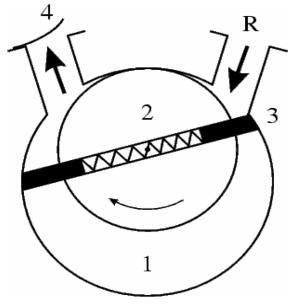
\includegraphics[scale=0.3]{content/images/Drehschieber.jpg}
\caption{Schematischer Aufbau einer Drehschieberpumpe \cite{Jena}.}
\label{fig:DSP}
\end{figure}